
% ****** Start of file apssamp.tex ******
%
%   This file is part of the APS files in the REVTeX 4.2 distribution.
%   Version 4.2a of REVTeX, December 2014
%
%   Copyright (c) 2014 The American Physical Society.
%
%   See the REVTeX 4 README file for restrictions and more information.
%
% TeX'ing this file requires that you have AMS-LaTeX 2.0 installed
% as well as the rest of the prerequisites for REVTeX 4.2
%n]
% See the REVTeX 4 README file
% It also requires running BibTeX. The commands are as follows:
%
%  1)  latex apssamp.tex
%  2)  bibtex apssamp
%  3)  latex apssamp.tex
%  4)  latex apssamp.tex
%
 
\documentclass[%
preprint,
%superscriptaddress,
%groupedaddress,
%unsortedaddress,
%runinaddress,
%frontmatterverbose, 
%preprint,
%preprintnumbers,
%nofootinbib,
%nobibnotes,
%bibnotes,
 amsmath,amssymb,
 aps,
 pra,
%prb,
%rmp,
%prstab,
%prstper,
%floatfix,
]{revtex4-2}

\newcommand{\revtex}{REV\TeX\ }
\newcommand{\classoption}[1]{\texttt{#1}}
\newcommand{\macro}[1]{\texttt{\textbackslash#1}}
\newcommand{\m}[1]{\macro{#1}}
\newcommand{\env}[1]{\texttt{#1}}
\setlength{\textheight}{9in}

\usepackage{graphicx}% Include figure files
\usepackage{dcolumn}% Align table columns on decimal point
\usepackage{bm}% bold math
\usepackage{floatrow}
\usepackage{comment}
\usepackage{mathrsfs}
\usepackage{xcolor}
\usepackage{hyperref}
\usepackage{cleveref}
\crefname{section}{§}{§§}
\Crefname{section}{§}{§§}
\hypersetup{
  colorlinks   = true, %Colours links instead of ugly boxes
  urlcolor     = blue, %Colour for external hyperlinks
  linkcolor    = blue, %Colour of internal links
  citecolor   = blue %Colour of citations
}

\begin{document}

\preprint{ }

\title{Mitigation of thermoacoustic instability in  a turbulent combustor via self-coupling }% Force line breaks with \\
% \thanks{A footnote to the article title}%

\author{Author1}\email{}\affiliation{Department of Aerospace Engineering, Indian Institute of Technology Madras, Chennai 600036, India}\author{Author2}\affiliation{Department of Aerospace Engineering, Indian Institute of Technology Madras, Chennai 600036, India}\author{Author3}\affiliation{Department of Aerospace Engineering, Indian Institute of Technology Madras, Chennai 600036, India}\author{Author4}\affiliation{Department of Aerospace Engineering, Indian Institute of Technology Madras, Chennai 600036, India}\author{Author5}\affiliation{Department of Aerospace Engineering, Indian Institute of Technology Madras, Chennai 600036, India}\author{Author6}\affiliation{Department of Aerospace Engineering, Indian Institute of Technology Madras, Chennai 600036, India}

%\author{Ankit Sahay, Amitesh Roy, Samadhan A. Pawar, R. I. Sujith}
% \altaffiliation[Also at ]{Physics Department, XYZ University.}%Lines break automatically or can be forced with \\
% \author{Ankit Sahay}%
% \email{ankitsahay02@gmail.com}
% \affiliation{Department of Aerospace Engineering, Indian Institute of Technology Madras, Chennai 600036, India}

\date{\today}% It is always \today, today,
             %  but any date may be explicitly specified
\begin{abstract}
In this paper, we report the first observation of complete mitigation of thermoacoustic instability in a bluff-body stabilized turbulent combustor through the method of self-coupling. Self-coupling is achieved by coupling the acoustic field of the combustor to itself through a coupling tube. We characterize the effects of such acoustic self-feedback on the dynamical behavior of the system for the variation of different parameters (length and diameter) of the coupling tube. We observe that the amplitude and the dominant frequency of the acoustic pressure fluctuations gradually decrease as the length of the coupling tube is increased, and complete suppression of thermoacoustic instability is observed when the coupling tube length is nearly 1.5 times the combustor length. Meanwhile, the dynamical behavior of these oscillations changes from limit cycle to chaos via intermittency. We also study the coupling between the acoustic field and the unsteady flame dynamics for different conditions of self-coupling in the combustor. As the combustor approaches the state of complete suppression, the temporal synchrony between the acoustic pressure and the global heat release rate signals changes from the state of synchronized periodicity to desynchronized chaos through intermittent synchronization. From the spatiotemporal analysis of the combustor flow field, we find complete disruption of the coherent spatial structures of acoustic energy production observed during the state of thermoacoustic instability, as these instabilities are suppressed through self-coupling in the combustor. Thus, we anticipate self-coupling to be a viable option to mitigate high amplitude thermoacoustic oscillations in turbulent combustion systems present in gas turbines and rocket engines.
\end{abstract}
%\keywords{Suggested keywords}%Use showkeys class option if keyword
                              %display desired
\maketitle

%\tableofcontents

\section{Introduction} \addvspace{10pt}

Thermoacoustic instabilities have proven to be a major deterrence to the development of low-emission gas turbine engines used for power generation and propulsion applications. These are ruinously large amplitude pressure oscillations established when a positive feedback is developed between the acoustic field and the heat release rate fluctuations in the reaction field of the combustor \cite{ sujith2021thermoacoustic}. These instabilities result in serious performance losses, structural degradation due to increased heat transfer, and reduced operational range \cite{culick2006unsteady}. As a result of potential harm to the structural integrity of a system, it is necessary to find ways to mitigate thermoacoustic instabilities in the course of developing new dynamically stable combustion systems.

Traditionally, different mechanisms of closed-loop and open-loop active controls have been developed for  suppressing thermoacoustic instability \cite{dowling2005feedback}. However, these methods suffer from several limitations, such as the use of complex electro-mechanical components, lack of reliability of sensors for operating in the harsh environment of practical combustors, and high maintenance and replacement costs. Another way to mitigate combustion instabilities is to use passive damping devices such as Helmholtz resonators, quarter-wave resonators, half-wave resonators \cite{zhao2015review}, and Herschel-Quincke tubes \cite{park2008thermo, rajaram2012attenuation}. Despite their limited range of operation, engine manufactures have to rely on these devises to suppress thermoacoustic instability in practical combustors \cite{bellucci2004use}. 

Recently, a method from synchronization theory, called mutual coupling of oscillators, has been adopted to suppress thermoacoustic instabilities in two or more systems \cite{sujith2021thermoacoustic}. At appropriate coupling parameters, the dynamical behavior of these coupled systems approach the same steady state, known as amplitude death in nonlinear dynamics parlance \cite{zou2021quenching}. Through experimental and numerical approaches, the presence of amplitude death and partial amplitude death has been extensively investigated in coupled laminar thermoacoustic systems \cite{thomas2018effect1, dange2019oscillation, hyodo2020suppression, srikanth2021dynamical}. In addition, a few studies have investigated the dynamics of mutually coupled turbulent combustors \cite{thomas2018effect, jegal2019mutual, moon2020mutual, guan2021low}, and have also reported the presence of amplitude death in them \cite{jegal2019mutual}. Here, the mutual coupling between the systems is achieved by using one (or more than one) tube of a fixed length and diameter. An increase in the length of the coupling tube correspondingly increases the delay time in the coupling of the acoustic fields in the systems \cite{dange2019oscillation, sahay2021dynamics}.

In contrast to the aforementioned studies, in this paper, we present the first application of a novel variant of mutual coupling, known as self-coupling, to mitigate thermoacoustic instabilities in a single turbulent combustion system. Here, the self-feedback is achieved by coupling the acoustic field of the combustor to itself, after a finite time delay, through a coupling tube of a specific length and diameter. This method has recently been used by a few researchers to suppress limit cycle oscillations in the acoustic field of different laminar systems such as electro-acoustic system \cite{biwa2016suppression}, acoustic pipeline \cite{lato2019passive}, and horizontal Rijke tube \cite{srikanth2021selfcoupling}. These studies have shown that subjecting a system to self-coupling affects its bifurcation characteristics \cite{srikanth2021selfcoupling}, where the suppression of acoustic pressure oscillations is realized only when a tube of a length equal to the odd multiple of the half-wavelength of the anticipated acoustic standing wave is used \cite{biwa2016suppression, lato2019passive}. Although these studies provide an understanding of the changes that happen in the acoustic field during mitigation of limit cycle oscillations in a self-coupled laminar system, this information might be insufficient to analyze the suppression of thermoacoustic instabilities in turbulent combustion systems. 

We know that thermoacoustic instabilities are a result of the complex interaction between the flow, the flame, and the acoustic field of a combustor \cite{sujith2021thermoacoustic}. As per the Rayleigh criterion, such instabilities occur only when in-phase synchrony is developed between two subsystems: the acoustic pressure and the heat release rate fluctuations in the combustor. Since the coupling between these subsystems plays a crucial role in the genesis of thermoacoustic instabilities, it is important to understand how the temporal and spatiotemporal coupling between these subsystems change during the suppression of thermoacoustic instability when the system is self-coupled. Towards this purpose, we systematically address the following questions in this paper \textendash  \hspace{0.5} (i) how effective is self-coupling in mitigating thermoacoustic instability in a turbulent combustor, (ii) what is the nature of the transition of acoustic pressure fluctuations during the suppression of thermoacoustic instability, and (iii) how does the temporal and spatiotemporal coupling between the acoustic pressure and heat release rate oscillations get affected due to self-coupling? 

To address these questions, we perform experiments on a laboratory-scale bluff-body stabilized turbulent combustor. We report the complete suppression of thermoacoustic instability in the combustor through self-coupling. We find that as the length of the coupling tube is changed, the amplitude and the frequency of acoustic pressure fluctuations exhibit a gradual decrease, and their dynamical behavior changes from the state of limit cycle oscillations to chaos via intermittency. We observe a lack of suppression of thermoacoustic instabilities when their amplitude prior to coupling is above a critical value for fixed parameters of the coupling tube. We also notice a gradual decay in the temporal synchrony between acoustic pressure and heat release rate fluctuations as the system dynamics approaches the complete state of suppression. Finally, we notice coherent regions of acoustic power production, due to local synchrony between acoustic pressure and heat release rate fluctuations, in the spatial field of the combustor during thermoacoustic instability. These coherent structures disintegrate during the transition to complete suppression of thermoacoustic instability.

\section{Experimental Setup} \addvspace{10pt}

\begin{figure}[t]
\centering
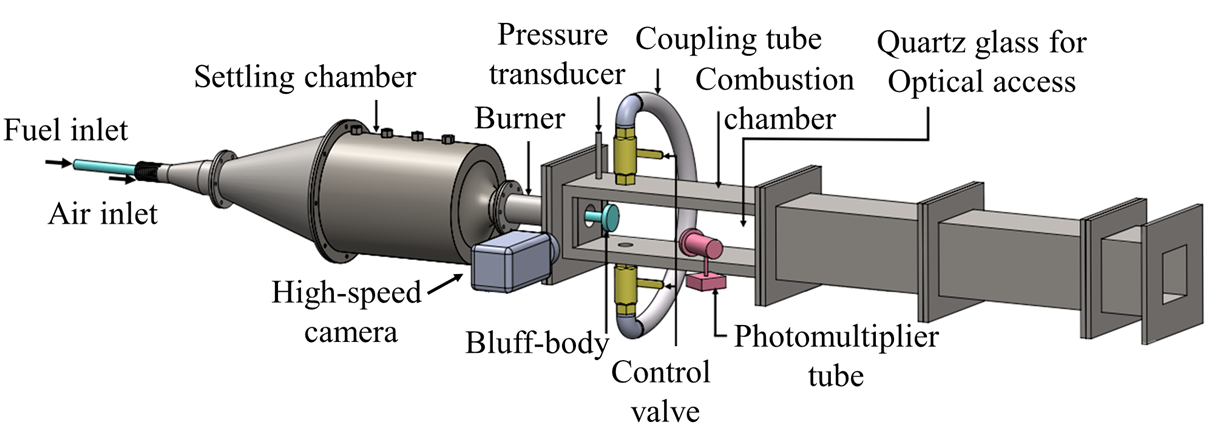
\includegraphics[width=0.9\textwidth]{fig1.png}
\caption{The schematic of a turbulent bluff-body stabilized combustor subjected to self-coupling using a single connecting tube.}
\label{TARA_fig}
\end{figure}
We experimentally demonstrate the application of self-coupling to mitigate thermoacoustic instability in a turbulent bluff-body stabilized dump combustor (Fig.~\ref{TARA_fig}). The combustor has a rectangular cross-section of $9 \times 9$ $\text{cm}^2$ and a length of $L_{\text{duct}} = 106$ $\text{cm}$. The experimental setup consists of a plenum chamber, a burner, a combustor, and an extended duct. Air at ambient conditions enters the plenum chamber, which ensures that the flow entering the combustor is immune to the upstream disturbances. The fuel (liquefied petroleum gas, 60\% butane and 40\% propane) is partially mixed in the air stream at the burner section prior to the combustor. Air and fuel flow rates are controlled through mass flow controllers. During experiments, we fix the fuel flow rate ($\dot{m_f}$) at a particular value and vary the air flow rate ($\dot{m_a}$) until thermoacoustic instability is established in the system. The Reynolds number of air flow is varied in the range of 14300 to 24500 throughout the experiments. We use a spark plug to ignite the partially premixed air-fuel mixture at the dump plane using an 11 kV ignition transformer. A disk-shaped bluff-body of thickness 1 cm and diameter 4.7 cm is used as the flame stabilizer and is positioned at 3 cm downstream of the dump plane. The combustion products are exhausted through a long duct into the atmosphere. 

Self-coupling is established in the combustor by feedbacking the acoustic of the combustor to itself using a single flexible stainless steel braided tube of length $L_c$ and internal diameter $d_c$ (refer to Fig.~\ref{TARA_fig}). The self-coupling tube is attached at an axial distance of 7 cm from the dump plane, on two opposite faces of the combustor walls, to achieve stronger acoustic feedback as it is near the anti-node of pressure standing wave in the system. Ball-type valves are manually operated to switch on and off the self-coupling of the acoustic field in the system. During self-coupling experiments, we first establish thermoacoustic instability of a particular amplitude in the system and then switch on the coupling by opening the valve.  

The acoustic pressure fluctuations $p^{\prime}(t)$ are measured using a PCB103B02 piezoelectric transducer (sensitivity: 217.5 mV/kPa and uncertainty: $\pm$0.15 Pa) mounted on the combustor wall at 2 cm from the dump plane. A photomultiplier tube (PMT, Hamamatsu H10722-01) equipped with a CH* filter (wavelength of 430 nm and 12 nm FWHM) is used to capture the global heat release rate fluctuations in the flame $\dot{q}^{\prime}(t)$. We simultaneously acquired both $p^{\prime}$  and $\dot{q}^{\prime}$  signals for 3 s at a sampling rate of 10 kHz using an A/D card (NI-6143, 16 bit). High-speed CH* chemiluminescence images of the flame are simultaneously captured with $p^{\prime}$  and $\dot{q}^{\prime}$ signals at 2000 fps for 3 s using a CMOS camera (Phantom - V12.1 with a ZEISS 50 mm camera lens). The image of the flow-field from the dump plane spans 9 cm $\times$ 12 cm with a resolution of 574 $\times$ 764 pixels.

\begin{figure}[t!]
\centering
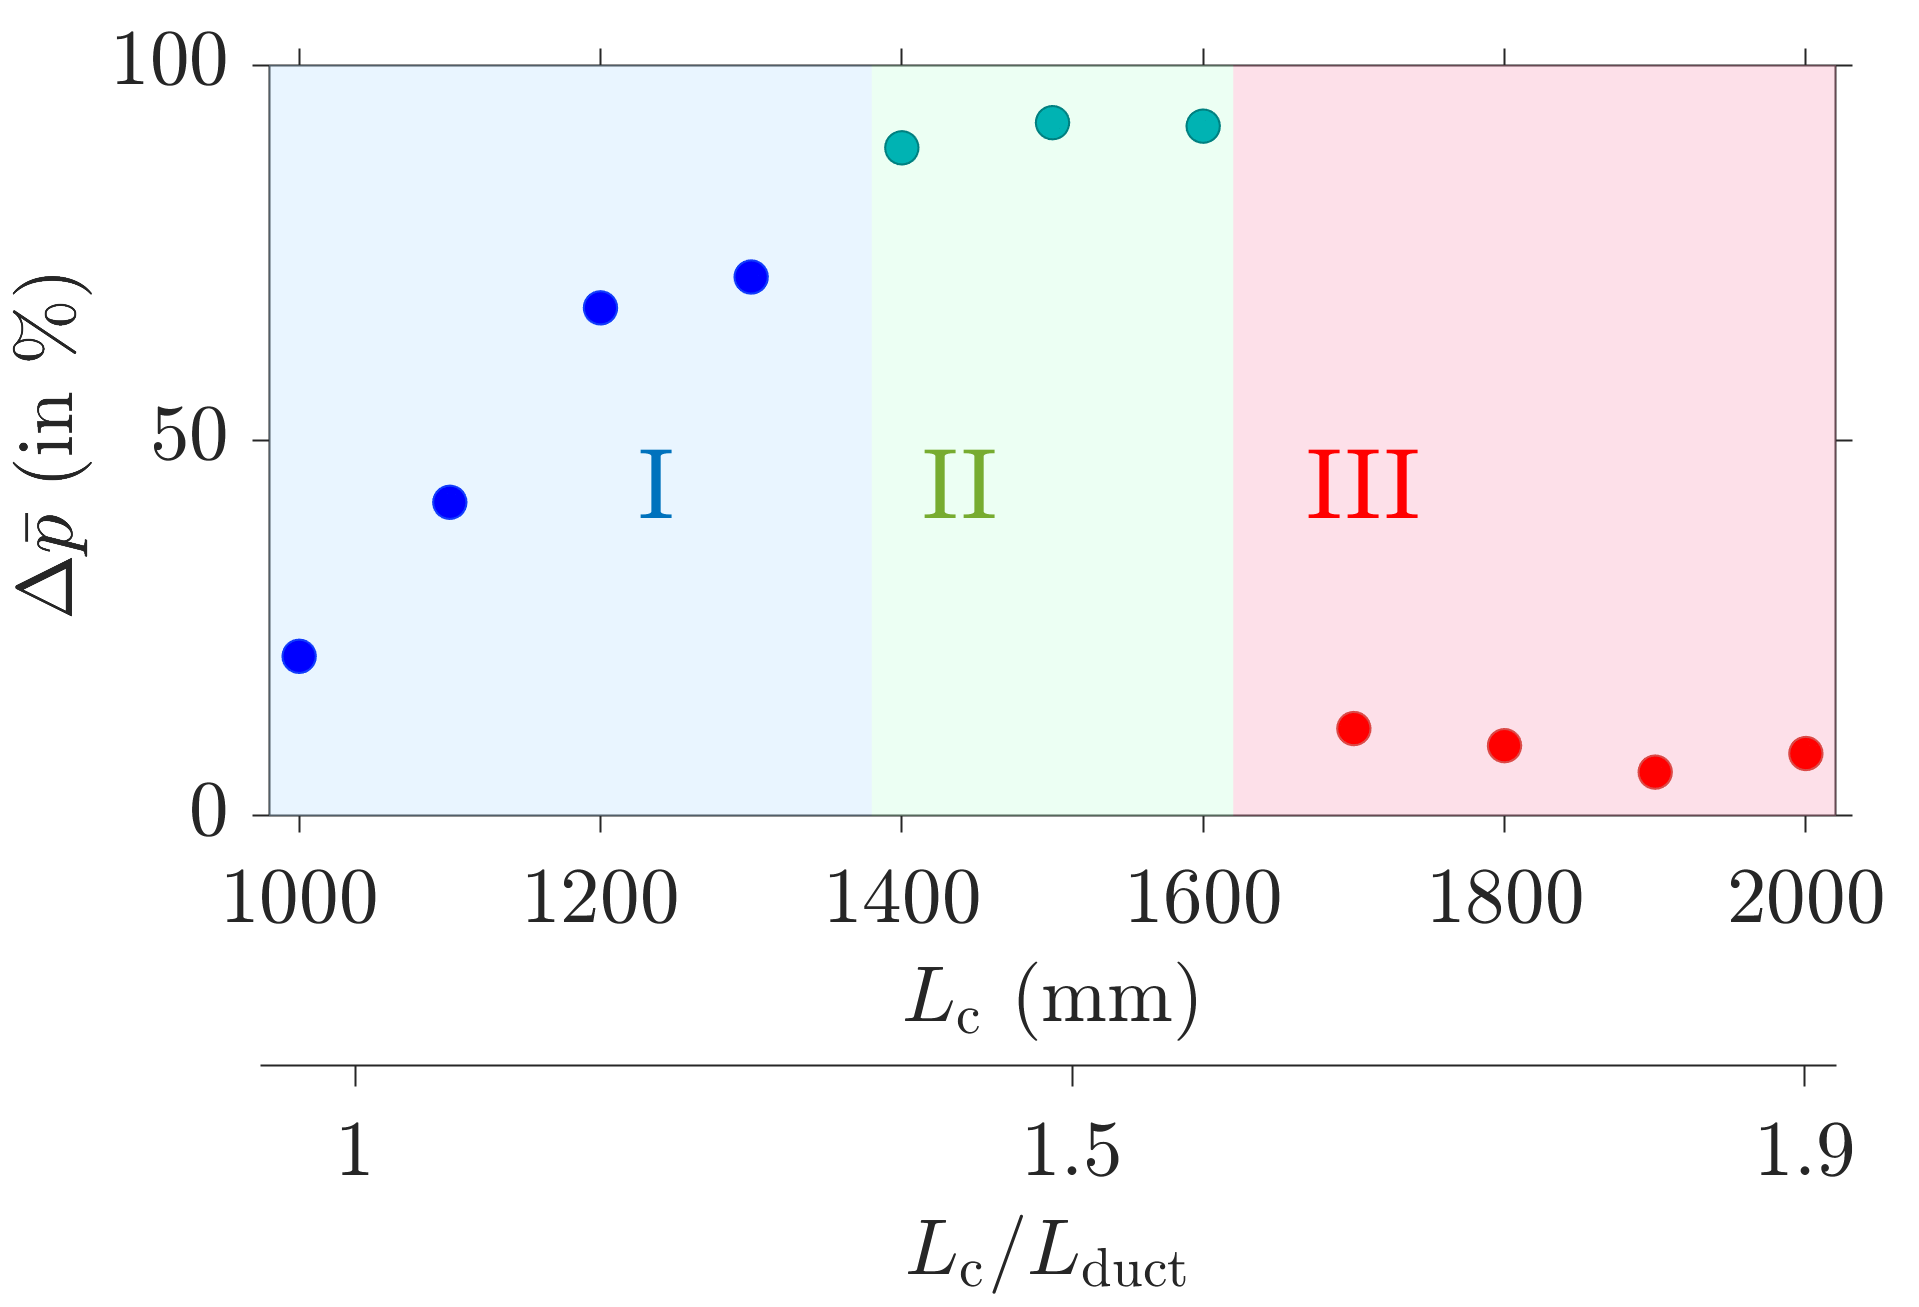
\includegraphics[width=.8\textwidth]{fig2.png}
\caption{The variation of $\Delta p^\prime_{rms}$ of self-coupled combustor with respect to increasing values of $L_c$. The regions marked I, II, and III denote the intermediate suppression, complete suppression, and no suppression, respectively, of thermoacoustic instability ($p^\prime_{0,rms}$) after self-coupling is induced in the combustor. The values of $L_{duct}$ and $d_c$ are fixed at 106 cm and 2.54 cm, respectively. }
\label{fig2}
\end{figure}

\section{Results and Discussion} \addvspace{10pt}

In this section, we systematically present the effect of self-coupling on the suppression of thermoacoustic instability in a turbulent combustor. We will first discuss temporal changes in the acoustic pressure signal ($p^{\prime}$) and then present changes in the coupled behavior of acoustic pressure and heat release rate fluctuations ($\dot{q}^{\prime}$) during the suppression of thermoacoustic instability in the self-coupled system.  

\subsection{Route from thermoacoustic instability to the state of complete suppression} \addvspace{10pt}
\begin{figure*}[t!]
\centering
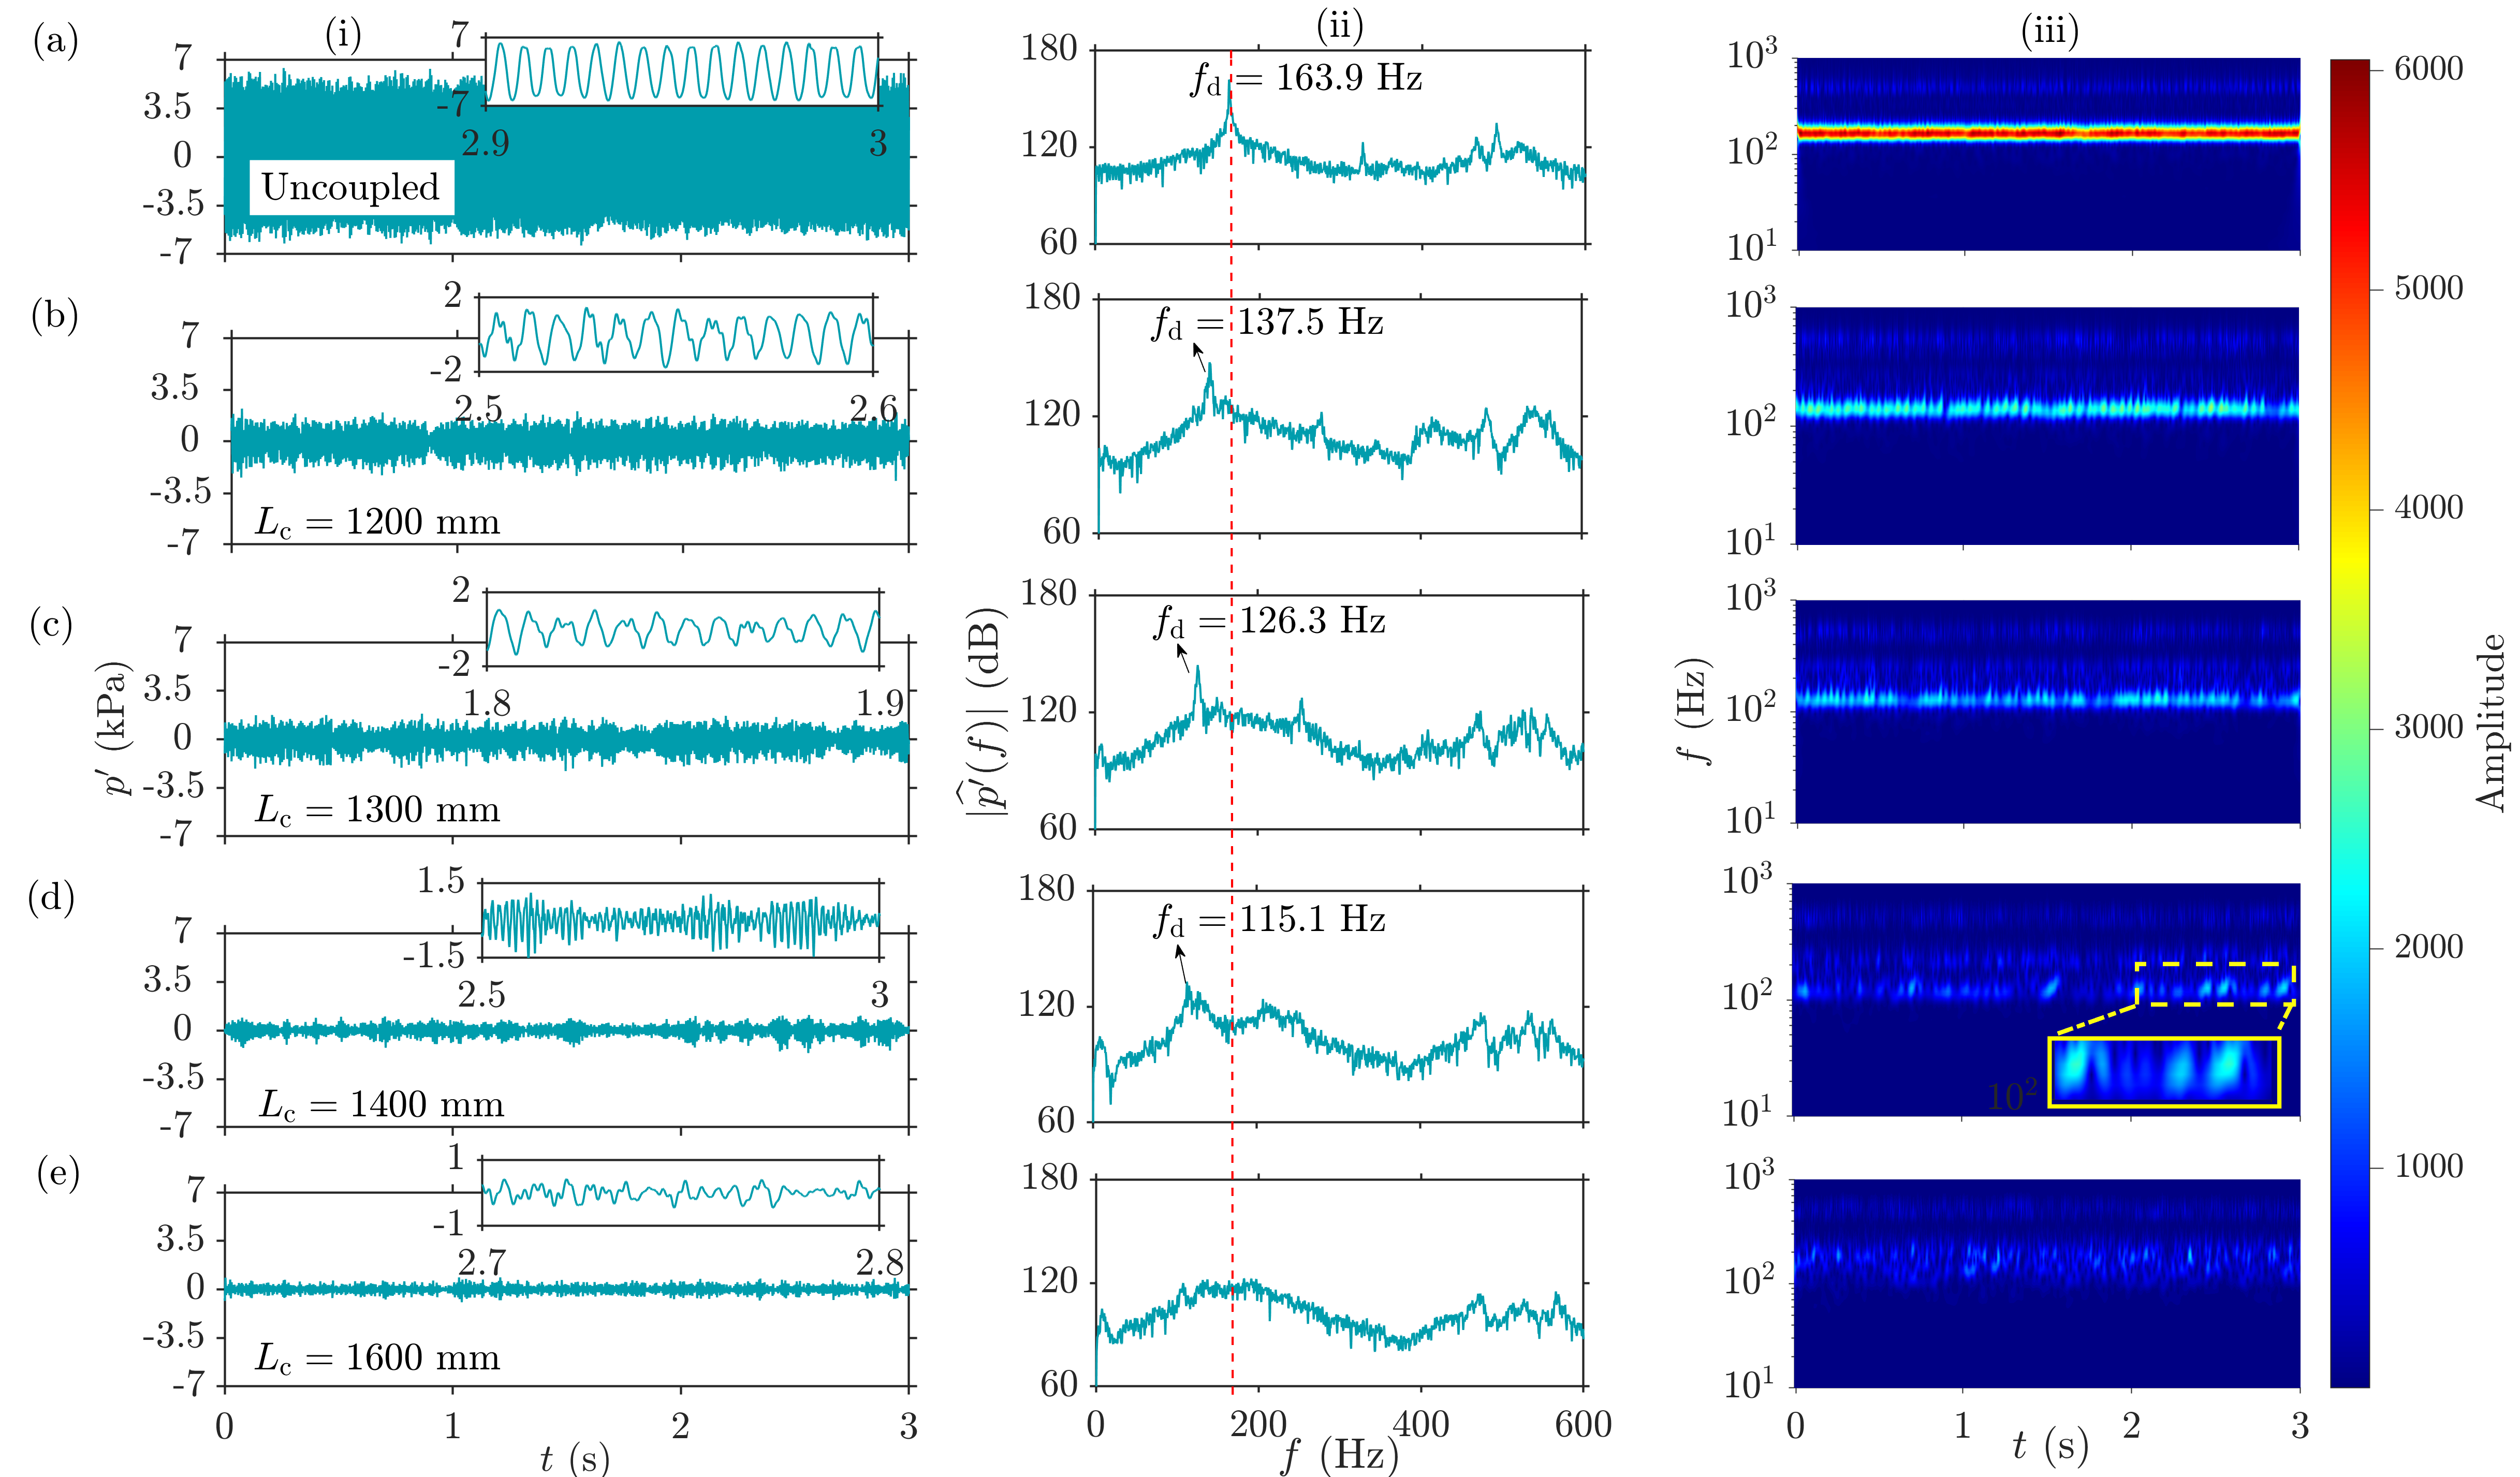
\includegraphics[width=1\textwidth]{fig3.png}
\caption{Variation of (i) time series, (ii) power spectral density, and (iii) scalograms of $p^\prime$ signals as the system behavior transitions from a state of (a) thermoacoustic instability to (e) complete suppression of oscillations via (b-d) intermittency. A vertical dotted red line in (ii) indicates the natural frequency of thermoacoustic instability observed in the absence of self-coupling. Zoomed regions of plots are shown in insets. The pink regions in the inset of (d)-iii shows the presence of periodic oscillations amidst blue regions of aperiodicity, thus indicating the presence of intermittency. $f_d$ denotes the dominant frequency in the power spectrum.
}
\label{fig3}
\end{figure*}

In Fig. \ref{fig2}, we show the percentage change in the root-mean-square (RMS) value of $p^{\prime}$ signals, i.e., $\Delta p^\prime_{rms}$, as a function of the length of the coupling tube ($L_c$) when its internal diameter is kept constant at 2.54 cm. $\Delta p^\prime_{rms}$ indicates the difference between the RMS values of $p^{\prime}$ signal during the state of thermoacoustic instability when the self-coupling is off and that of $p^{\prime}$ signals when the self-coupling is switched on, i.e., $\Delta p^\prime_{rms} = p^\prime_{0,rms}-p^\prime_{rms}$. The value of $\Delta p^\prime_{rms}$ is further normalized by $p^\prime_{0,rms}\approx 3200$ Pa. 

We notice a gradual decrease in the amplitude of $p^{\prime}$ signal with an increase in $L_c$ during the complete suppression thermoacoustic instability in the system. However, post the region of complete suppression, i.e., at higher values of $L_c$, $\Delta p^\prime_{rms}$ dips suddenly to a lower value as the amplitude of $p^\prime$ oscillations are nearly unaffected by self-coupling. During the state of complete suppression, we note that the amplitude of $p^{\prime}$ signal is comparable to that of observed for the state of stable operation (i.e., combustion noise). Furthermore, the optimum value $L_c$ corresponding to the complete suppression of thermoacoustic instability is observed to be approximately 1.5 times the length of the combustor (i.e., $L_c/L_{\text{duct}} \approx 1.5$).

 Figure ~\ref{fig3} shows the changes in the characteristics of $p^{\prime}$ signal, plotted in terms of time series, power spectrum, and scalogram, in the absence of coupling (Fig.~\ref{fig3}a) and when the system is self-coupled for different lengths of the coupling tube (Fig.~\ref{fig3}b-e). In the absence of self-coupling, during thermoacoustic instability (Fig.~\ref{fig3}a), we observe large amplitude periodic oscillations in the time series (Fig.~\ref{fig3}a-i), a sharp spectral peak at 163.9 Hz corresponding to the fundamental mode of the combustor in the power spectrum (Fig.~\ref{fig3}a-ii), and a continuous distribution of the spectral power throughout the time in a narrow frequency band in the scalogram (Fig.~\ref{fig3}a-iii).

As soon as self-coupling is established in the combustor, we notice a significant change in the properties of $p^{\prime}$ signals. On increasing $L_c$, the dynamical behavior of $p^{\prime}$ changes from the state of large amplitude periodic oscillations (Fig.~\ref{fig3}a) to low amplitude chaotic oscillations (Fig.~\ref{fig3}e ) via intermittent oscillations (Fig.~\ref{fig3}c,d). During intermittent oscillations, regions of low amplitude chaotic fluctuations separate regions of large amplitude periodic oscillations in an apparently random manner (see inset in Fig.~\ref{fig3}d-iii). The existence of chaos during the state of complete suppression of thermoacoustic instability is confirmed by carrying out the well-known 0-1 test of chaos \cite{gottwald2004new}. The results of the 0-1 test of chaos are presented in the Supplementary Material. This chaotic property of $p^{\prime}$ signal during the state of suppression is similar to that observed for the state of stable operation by Nair \textit{et al.} \cite{nair2013loss} in the same combustor. 

\begin{figure*}[t!]
\centering
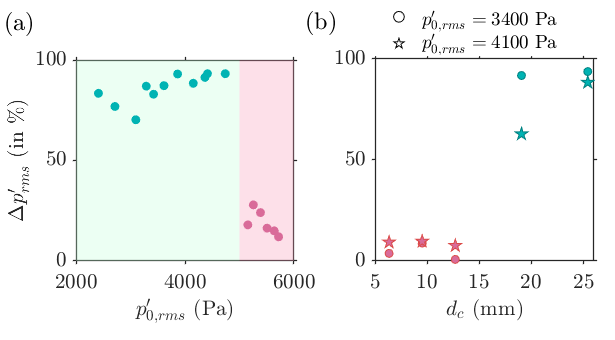
\includegraphics[width=0.9\textwidth]{diff_amp_and_dia.png}
\caption{The percentage suppression of acoustic pressure signals ($\Delta p^\prime_{rms}$) when self-coupling is applied (a) to thermoacoustic instability of different amplitudes ($p^\prime_{0,rms}$) for constant values of $L_{c} = 140$ cm and $d_c = 2.54$ cm, and (b) to thermoacoustic instability of nearly the same amplitude  ($p^\prime_{0,rms} \approx 3.4$ kPa) for different coupling tube diameters ($d_c$) at a fixed value of $L_c = 140$ cm. \textcolor{red}{Fig. b will be revised to have more points; we are conducting experiments.}}
\label{diff_amp_dia}
\end{figure*}

Furthermore, we notice a gradual decrease in the value of the dominant frequency and the corresponding spectral amplitude in the power spectrum of acoustic pressure fluctuations during the suppression of thermoacoustic instability (compare plots in Fig.~\ref{fig3}a-ii to Fig.~\ref{fig3}e-ii). The scalogram plots during this transition show an increase in interruptions in the dominant spectral power of the signal (Fig.~\ref{fig3}b-iii to Fig.~\ref{fig3}d-iii), and these interruptions are highly frequent during the state of complete suppression of thermoacoustic instability (Fig.~\ref{fig3}e-iii). Thus, we observe that both the temporal and spectral properties of acoustic pressure fluctuations exhibit a gradual change during the mitigation of thermoacoustic instability in a self-coupled turbulent combustor.

Next, we examine the effect of self-coupling on the suppression of  thermoacoustic instability of different amplitudes ($p^\prime_{0,rms}$) for $L_c=140$ cm and $d_c=2.54$ cm (Fig. \ref{diff_amp_dia}a). Here, the amplitude of thermoacoustic before initiating self-coupling is varied primarily by changing the fuel flow rate in the combustion mixture. We observe that thermoacoustic instability of low amplitudes (i.e., $p^\prime_{0,rms} \leq 5$ kPa, region $\text{I}$ in Fig. \ref{diff_amp_dia}a) can be completely suppressed with the given coupling tube, while thermoacoustic instabilities of larger amplitudes (i.e., $p^\prime_{0,rms} > 5$ kPa, region $\text{II}$ in Fig. \ref{diff_amp_dia}a) are not quenched with this coupling tube. In this region, we observe a small decrease in the amplitude of thermoacoustic instability due to self-coupling. Thus, we infer that a coupling tube with optimal parameters can mitigate thermoacoustic instability lesser than a certain critical value of $p^\prime_{0,rms}$. Furthermore, by performing experiments for different diameters of the coupling tube ($d_c$), for a fixed value of $L_c$ (Fig. \ref{diff_amp_dia}b), we found that the suppression of thermoacoustic instability in a system also depends on $d_c$, where a larger diameter coupling tube can quench thermoacoustic instability of higher amplitude for a fixed $L_c$. These results are consistent with that observed in a self-coupled laminar thermoacoustic system by Srikanth \textit{et al.} \cite{srikanth2021selfcoupling}.

\subsection{Temporal analysis of coupled acoustic pressure and global heat release rate fluctuations}

In this section, we investigate the change in the coupled behavior of the acoustic pressure ($p^{\prime}$) and the global heat release rate ($\dot{q}^{\prime}$) fluctuations during the suppression of thermoacoustic instability, by examining the locking of their instantaneous phases and frequencies (Fig.~\ref{fig4}). The phase and frequency locking (i.e., synchronization) of such signals can be analyzed using a cross-wavelet transform plot \cite{grinsted2004application}. In this plot, the regions of common spectral power for both the signals in time are highlighted by a brighter color, and the corresponding wrapped instantaneous relative phases between them are indicated by arrows. When the signals are synchronized in time, their cross wavelet transform shows a larger magnitude of the spectral power throughout the signal and a constant alignment of arrows at a particular phase difference. In contrast, desynchronization of signals is indicated in the cross wavelet transform plot by a near random distribution of the common spectral power and an arbitrary alignment of arrows in time.

\begin{figure*}[t!]
\centering
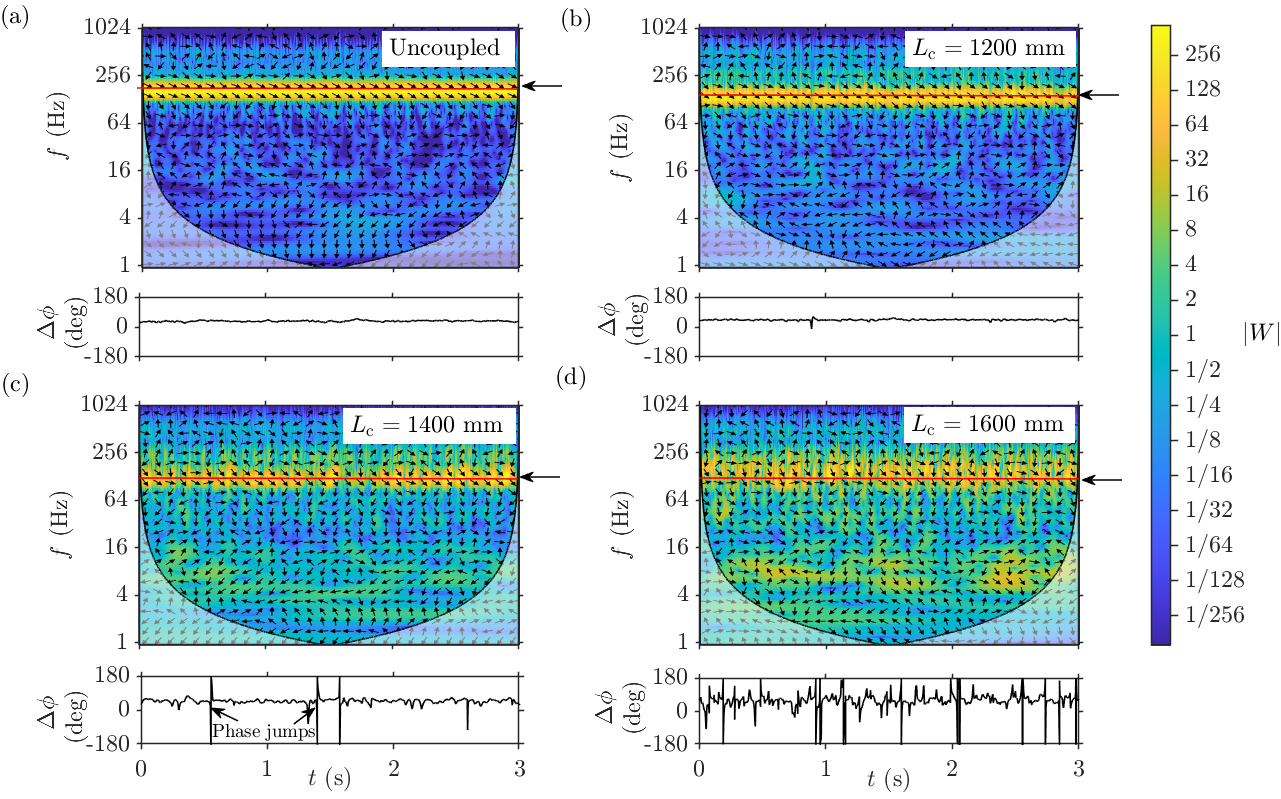
\includegraphics[width=0.9\textwidth]{all_copy.png}
\caption{Cross wavelet transform plots between $p^\prime$ and $\dot{q}^\prime$ signals and the temporal variation of their phase difference $\Delta\phi$, calculated at the dominant frequency (indicated by a horizontal red dotted line and an arrow in each cross wavelet transform plot), for (a) the state of thermoacoustic instability in the absence of self-coupling and (b-d) for the states of self-coupled combustor with increasing values of $L_c$. The value of $d_c$ is kept constant at 2.54 cm. }
\label{fig4}
\end{figure*}

\begin{table*}[!b] \small
\centering
\caption{\label{table} Phase Locking Value (PLV) and Pearson's correlation coefficient ($\rho$) between $p^\prime$ and $\dot{q}^\prime$ for different $L_c$.}
\begin{tabular}{|l|l|l|l|l|l|l|l|l|l|l|l|l|}
\hline
$L_c$ (in cm)                   & 100  & 110  & 120  & 130  & 140  & 150  & 160  & 170  & 180  & 190  & 200  & 215  \\
\hline
PLV                 & 0.97 & 0.96 & 0.91 & 0.84 &   -   &    -  &   -   & 0.94 & 0.93 & 0.95 & 0.91 & 0.93 \\
\hline
$\rho$ & 0.64 & 0.62 & 0.65 & 0.60 & 0.41 & 0.37 & 0.25 & 0.55 & 0.55 & 0.69 & 0.64 & 0.59 \\
\hline
\end{tabular}
\label{table}
\end{table*}

In Fig. \ref{fig4}a, we notice that both $p^{\prime}$ and $\dot{q}^{\prime}$ signals are perfectly synchronized at a frequency of 163.9 Hz, where the relative phase ($\Delta\phi$) between them stays constant around $35.3^\circ$. When the system is self-coupled for $L_c = 120$ cm, in the regime of intermediate suppression (Fig. \ref{fig2}), we observe the appearance of a common frequency band around the dominant frequency of 131.5 Hz for almost the entire duration of the signal (Fig.~\ref{fig4}b). The variation of $\Delta\phi$ at 131.5 Hz is nearly constant around a mean value of $42.7^\circ$ throughout the signal except for a small phase jump observed at a particular time instance when the signals are momentarily desynchronized. As the length of the coupling tube $L_c$ is increased to 140 and 160 cm (see Fig.~\ref{fig4}c and Fig.~\ref{fig4}d, respectively), we notice a corresponding increase in the discontinuities in the common frequency bands of these signals. This increase in discontinuities of common frequency regions can be easily seen from the plots of $\Delta\phi$, where we notice an increase in the number of phase jumps about a mean phase difference for these signals. This behavior of the temporal variation of $\Delta\phi$ can be associated with the increase in the duration of desynchronization of $p^{\prime}$ and $\dot{q}^{\prime}$ oscillations in the system. We find that these instances of desynchronized oscillations coincide with low amplitude chaotic oscillations observed in $p^{\prime}$ and $\dot{q}^{\prime}$ signals. During the state of suppression of thermoacoustic instability (i.e., for $L_c = 160$ cm in Fig. \ref{fig4}d), we notice complete desynchronization of $p^{\prime}$ and $\dot{q}^{\prime}$ signals in the system. This happens when the sustained positive feedback between these oscillations is entirely destroyed. 

In addition, we use two quantifiers, called phase locking value (PLV) and Pearson's correlation coefficient ($\rho$), to detect the synchronization behavior of $p^{\prime}$ and $\dot{q}^{\prime}$ signals for different values of $L_c$ shown in Fig. \ref{fig2}. PLV helps us to detect phase synchronization between two signals and is calculated as PLV = $(1/N) \Big{\lvert} \sum\limits_{n=1}^N \text{exp}(i \Delta \phi) \Big{\lvert}$ \cite{pikovsky2001universal}, where $N$ is the number of data points in a signal. On the other hand, $\rho$ aids in finding the amplitude correlation between the signals \cite{gonzalez2002amplitude}, and is calculated as $\rho = \text{Cov}(p^{\prime},\dot{q}^{\prime})/(\sigma_{p^{\prime}} \times \sigma_{\dot{q}^{\prime}})$. Here, $\sigma$ denotes the standard deviation of a signal, and $\text{Cov}$ represents the covariance between two signals. We have presented the values of these measures in Table \ref{table}. We find that in the regime of intermediate suppression of thermoacoustic instability, both $p^{\prime}$ and $\dot{q}^{\prime}$ are phase synchronized, confirmed from the PLV near 1. Inside the regime of suppression, as the signals are aperiodic where the phase of the oscillations is not physically defined, we do not calculate PLV \cite{pikovsky2001universal,sujith2021thermoacoustic}. The value of $\rho$ is observed to be highly positive (between 0.55 and 0.7) in the regime of oscillatory state, while it drops to 0.25 in the regime of suppression of thermoacoustic instability, which happens due to the lack of amplitude correlation between desynchronized signals.   

Thus, we observe that the extent of synchronization of the coupled $p^{\prime}$ and $\dot{q}^{\prime}$ signals decreases during the mitigation of thermoacoustic instability in a turbulent combustor, where the coupled behavior of these signals changes from the state of synchronized periodicity to desynchronized chaos via intermittent synchronized oscillations.

\subsection{Spatiotemporal analysis during the complete suppression of thermoacoustic instability} \addvspace{10pt}
\begin{figure*}[t!]
\centering
\includegraphics[width=0.85\textwidth]{spatio_temporal_5.png}
\caption{Time series of $p^{\prime}$ and $\dot{q}^{\prime}$ and the corresponding (i-viii) phase-averaged images of instantaneous distribution of acoustic power $p^\prime(t)\dot{q}^\prime(x,y,t)$ for the states of (a) thermoacoustic instability and (b) the complete suppression of these instabilities.}
\label{fig5}
\end{figure*}
In this section, we compare the spatiotemporal changes in the combustor as thermoacoustic instabilities are suppressed through self-coupling. During the state of thermoacoustic instability, we notice the periodic emergence of large-scale vortical structures from the dump plane of the combustor (shown in Fig. S2 of Supplementary Material). These vortices impinge on both the side walls of the combustor and the bluff-body. The breaking of these vortices results in the fine scale mixing of the reactants and hot products, causing a large heat release release fluctuations in the system. In contrast, during the state of complete suppression of thermoacoustic instability, we observe the absence of any such large-scale vortex in the combustor, wherein the flame dynamics appears to be nearly the same at all time instances. 

In Fig. \ref{fig5}a(i-viii), we show the spatial distribution of $p^\prime(t) \dot{q}^\prime(x,y,t)$, i.e., local acoustic power, calculated for the phase-averaged images corresponding to the state of thermoacoustic instability. Such phase-averaged images are not shown for the state of complete suppression as the signals are aperiodic in time; as a result, we show eight representative snapshots of instantaneous distribution of local acoustic power for this state in Fig. \ref{fig5}b(i-viii). The blue color in Fig. \ref{fig5}(i-viii) represents the local acoustic power sinks ($p^\prime(t) \dot{q}^\prime(x,y,t)$ $<0$), whereas the red color represents the local acoustic power sources ($p^\prime(t) \dot{q}^\prime(x,y,t)$ $>0$).

During the state of thermoacoustic instability, we observe larger coherent regions of  acoustic power sources on the top and downstream of the bluff-body. When both $p^\prime$ and $\dot{q}^\prime$ signals are near their local maxima (Fig. \ref{fig5}a(i,ii)), these regions of acoustic power sources consist of larger magnitude and are observed in terms of clusters in the spatial field. On the other hand, when both $p^\prime$ and $\dot{q}^\prime$ signals are near their local minima (Fig. \ref{fig5}a(v,iv)), acoustic power sources appear to be of low magnitude and nearly  spread over the entire combustor flow field. The local acoustic power distribution is near zero when the phase of the signal is near 0 or 180 deg (Fig. \ref{fig5}a(iii,vii), respectively). Small regions of acoustic power sink are observed around the shaft of the bluff-body. Thus, the local distribution of acoustic power is highly dynamic during the state of thermoacoustic instability. 

During the state of complete suppression of thermoacoustic instability (Fig. \ref{fig5}b(i-viii)), we observe that the spatial distribution of instantaneous acoustic power is highly inhomogeneous (incoherent), and its value is observed to be in negative (acoustic power sinks) in the majority of the reaction field of the combustor. Therefore, we notice that the self-acoustic coupling of the combustor using a coupling tube of optimum length and diameter breaks the constructive interactions between the acoustic pressure and the local heat release rate oscillations, which causes lesser driving from the heat release rate field to the acoustic field of the combustor. As a result, the suppression of thermoacoustic instability is observed in the system.

\section{Conclusion} \addvspace{10pt}

In summary, we demonstrate the possibility of complete mitigation of thermoacoustic instability in a bluff-body stabilized turbulent combustor by inducing a delayed acoustic self-feedback in the system. This self-feedback is achieved by coupling the acoustic field of the system to itself, using a tube attached near the anti-node position of the acoustic standing wave. We observe complete suppression of thermoacoustic instability in the combustor when the length of the coupling tube is approximately 1.5 times that of the combustor (i.e., $L_c \approx 1.5L_{duct}$). We find that the mitigation of these instabilities is associated with a gradual decrease in the amplitude of acoustic pressure oscillations and a shift in their dominant frequency towards a lower value. Furthermore, we notice that the dynamical behavior of acoustic pressure fluctuations changes from the state of limit cycle oscillations to chaotic oscillations via intermittent oscillations during the suppression of thermoacoustic instability. The synchronization of the acoustic pressure and global heat release rate fluctuations, observed during the uncoupled state of thermoacoustic instability, breaks down gradually and the oscillations become desynchronized as the system approaches the state of complete suppression. During this state, we do not observe any large-scale coherent structures in the reaction field of the combustor as witnessed during thermoacoustic instability. We also notice the disruption of acoustic power sources in the reaction during the state of complete suppression of oscillations, which happens due to the breaking of the local synchrony between acoustic pressure and heat release rate fluctuations in the spatial field of the combustor. 

Thus, self-coupling provides a promising control mechanism to suppress thermoacoustic instability in turbulent combustors. Unlike in traditional active closed-loop controls, we do not need to preprocess the pressure signal using any electromechanical devices in the method of self-coupling. Therefore, we believe that self-coupling opens up novel, cost-effective ways to mitigate thermoacoustic instability in practical gas turbines and rocket engines. 

\section*{Acknowledgments}
% This work is supported by the Office of Naval Research Global (Contract Monitor: Dr R. Kolar) under Grant No. N62909-18-1-2061.
This work is supported by the IoE initiative
(SB/2021/0845/AE/MHRD/002696) from the Department of Science and Technology (DST), Government of India.

\bibliographystyle{apsrev4-2}
\bibliography{PCI_LaTeX.bib}% Produces the bibliography via BibTeX.


\end{document}
%
% ****** End of file apssamp.tex ******
